\chapter{Introduzione}\label{cap:introduzione}

\section{L'azienda}

Sync Lab (logo in figura \ref{fig:logo-synclab}) è una \textit{software house} italiana nata a Napoli nel 2002 che, grazie ad una progressiva
maturazione delle sue competenze in ambito applicativo e tecnologico, è riuscita a diventare un
punto di riferimento per le aziende che intendono innovare i propri processi di business,
trasformandosi in un \textit{System Integrator}. L'azienda si è fatta notare sul mercato grazie alla proposta
di vari prodotti software, sviluppati all'interno del suo laboratorio di ricerca e sviluppo, 
conquistando importanti fette di mercato in ambito nazionale nei settori mobile, di sicurezza e videosorveglianza.
Ad oggi, Sync Lab conta più di 150 clienti e oltre 200 dipendenti dislocati nelle proprie sedi.
Queste sono situate a Napoli, Milano, Verona, Roma e Padova.
L'obiettivo principale dell'azienda è quello di fornire soluzioni tecnologiche innovative e di qualità
che possano soddisfare le esigenze dei propri clienti, garantendo un servizio di consulenza
e assistenza continuo e di alto livello.\\

\begin{figure}[h]
    \centering
    
\includegraphics[width=0.4\textwidth, alt={Logo dell'azienda Sync Lab}]{immagini/synclab.png}
    \caption{Logo azienda Sync Lab}\label{fig:logo-synclab}
\end{figure}

\newpage

\section{Way of Working e strumenti}
L'azienda Sync Lab adotta un modello di sviluppo \glsfirstoccur{\gls{agileg}}, con l'obiettivo di monitorare e controllare lo sviluppo del progetto in modo flessibile e continuo, suddividendo le attività
in piccoli incrementi e con una collaborazione asincrona e distribuita. In particolare, il modello di sviluppo adottato è \glsfirstoccur{\gls{scrumg}}, che prevede la suddivisione del progetto in sprint,
ovvero periodi di tempo di durata fissa, in cui vengono pianificate le attività da svolgere e i relativi obiettivi da raggiungere. Al termine di ogni sprint, viene effettuato su base settimanale
un incontro interno approfondito con il tutor aziendale, per discutere lo stato di avanzamento del progetto e le attività da svolgere per il successivo sprint. \\

L'obiettivo del modello è dare maggiore importanza al ciclo di vita del \glsfirstoccur{\gls{softwareg}} e dei processi correlati, piuttosto che al prodotto finale, con l'obiettivo di migliorare la qualità del prodotto stesso.
Inoltre, grazie alla collaborazione con altri stagisti con progetti basati sugli stessi concetti e in generale con il team di sviluppo, è stato possibile condividere conoscenze e competenze,
discutere problemi e trovare soluzioni comuni, con un approccio incrementale e iterativo. \\

Gli strumenti utilizzati per lo sviluppo del progetto sono stati i seguenti:
\begin{itemize}
    \item{\textit{\textbf{Trello}}}, per la gestione delle attività e dei task da svolgere (esempio in figura  \ref{fig:trello}), condiviso con il tutor aziendale e verificato dallo stesso ad ogni incremento.
    All'interno di questo strumento è possibile monitorare le attività attraverso delle schede, simili a dei \textit{post-it}, differenziando le attività per specifiche colonne di avanzamento.
    Le diciture riportate dalle colonne sono generalmente come segue:
    \begin{itemize}
        \item{\textbf{Backlog}}: che contiene attività in corso di svolgimento, comprendenti schede con obiettivi di massima dello stage e delle sue singole parti e periodi;
        \item{\textbf{In corso}}, ossia attività in esecuzione e da realizzare entro la fine dello \textit{sprint};
        \item{\textbf{In verifica}}, ossia attività in attesa di verifica e considerate concluse, in attesa di essere spostate nella colonna \textit{Terminati} a seguito della \textit{sprint review};
        \item{\textbf{Terminati}}, cioè attività completate e verificate da parte del tutor aziendale.
    \end{itemize} 
    \begin{figure}[h]
        \centering
        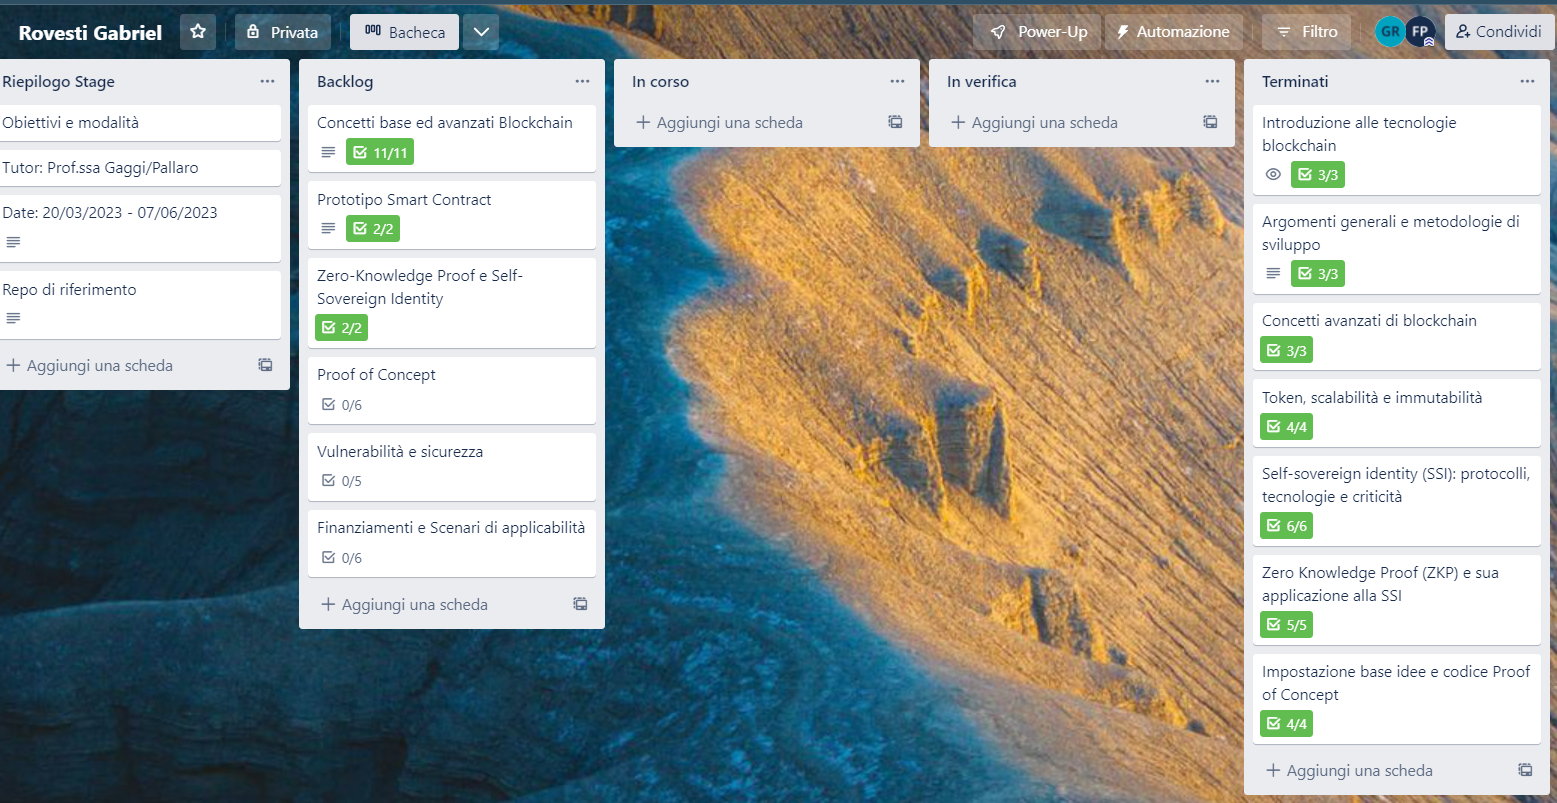
\includegraphics[width=1\textwidth, alt={Esempio di utilizzo di Trello}]{immagini/trello.png}
        \caption{Esempio di utilizzo di Trello}\label{fig:trello}
    \end{figure}

    \item{\textit{\textbf{Google Calendar}}}, per la pianificazione delle attività e degli incontri con il tutor aziendale, condiviso con il tutor stesso e con gli altri stagisti 
    e dipendenti di Sync Lab, capendo così e in anticipo le attività da svolgere e gli incontri da effettuare;
    
    \item{\textit{\textbf{Visual Studio Code}}}, \glsfirstoccur{\gls{ideg}} utilizzato per la scrittura del codice sorgente e dei file di configurazione, con l'aggiunta di alcuni \textit{plugin} per la formattazione del codice e per la gestione dei file di configurazione 
    del progetto. All'interno di questo, è stato realizzato lo studio di esempi di codice e la realizzazione dell'intero progetto, con l'aggiunta di un sistema di \textit{linting} per la formattazione del codice e di un sistema di \textit{debugging} per il controllo del flusso di esecuzione del codice.
    Sempre tramite questo strumento, è stata scritto la tesi, attraverso l'utilizzo di un \textit{plugin} per la scrittura in \LaTeX;
    
    \item{\textit{\textbf{Diagrams.net}}}, per la realizzazione e la creazione delle immagini del documento, utilizzati per la documentazione e la strutturazione delle sezioni;
    
    \item{\textit{\textbf{StarUML}}}, per la realizzazione dei diagrammi \glsfirstoccur{\gls{umlg}} del documento, quindi per i diagrammi dei casi d'uso e dei diagrammi delle classi;

    \item{\textit{\textbf{GitHub}}}, utilizzato internamente per la gestione del codice sorgente e dei file di configurazione, condiviso con il tutor aziendale e verificato dallo stesso ad ogni incremento.
    In particolare, è stato utilizzato il sistema di controllo versione \glsfirstoccur{\gls{gitg}}, che permette di tenere traccia delle modifiche effettuate ai file e di gestire le varie versioni del codice e degli appunti interni 
    da me realizzati, per una migliore organizzazione e condivisione delle informazioni. Inoltre, è stato possibile condividere il codice sorgente con gli altri stagisti e dipendenti di Sync Lab,
    per garantire il versionamento e la condivisione delle modifiche effettuate.
    
    \item{\textit{\textbf{Discord}}}, social network utilizzato per la comunicazione interna tra i dipendenti di Sync Lab, 
    tramite la gestione di vari canali vocali e testuali divisi per argomento e per sedi interne aziendali. La suddivisione in gruppi e canali
    ha permesso di comunicare in modo efficace e veloce, condividendo informazioni e risorse utili per lo svolgimento del progetto, sia a livello di risorse 
    didattiche che per la risoluzione di eventuali dubbi e problemi. Inoltre, è stato possibile comunicare con gli altri stagisti in modo semplice e veloce,
    condividendo conoscenze e competenze e discutendo problemi e soluzioni comuni.
\end{itemize}

\section{Organizzazione del testo}

\subsection{Struttura del documento}

\begin{description}
    \item[{\hyperref[cap:tecnologie]{Il secondo capitolo}}] descrive le tecnologie studiate e utilizzate per lo sviluppo del progetto.
    
    \item[{\hyperref[cap:descrizione-stage]{Il terzo capitolo}}] approfondisce il percorso di tirocinio formativo, descrivendo precisamente gli obiettivi e le attività svolte durante il percorso,
    con relativa analisi dei rischi.
    
    \item[{\hyperref[cap:analisi-requisiti]{Il quarto capitolo}}] approfondisce il progetto da un punto di vista tecnico, descrivendo i requisiti e i casi d'uso del progetto.
    
    \item[{\hyperref[cap:progettazione-codifica]{Il quinto capitolo}}] approfondisce le tecnologie utilizzate per la realizzazione del progetto, descrivendo le scelte progettuali e le soluzioni implementate,
    a livello architetturale e di codifica.
    
    %\item[{\hyperref[cap:verifica-validazione]{Il sesto capitolo}}] approfondisce le attività di verifica e validazione del progetto, descrivendo le tipologie di test effettuate e i risultati ottenuti.
    %
    %\item[{\hyperref[cap:conclusioni]{Nel settimo capitolo}}] descrive lo stato degli obiettivi raggiunti e la valutazione personale del percorso, con un'analisi retrospettiva del progetto e del suo utilizzo
    % rispetto a sviluppi futuri sulle stesse tematiche.
\end{description}

\subsection{Convenzioni tipografiche}
Riguardo la stesura del testo, relativamente al documento sono state adottate le seguenti convenzioni tipografiche:
\begin{itemize}
	\item gli acronimi, le abbreviazioni e i termini ambigui o di uso non comune menzionati vengono definiti nel glossario, situato alla fine del presente documento;
	\item i termini in lingua straniera o facenti parti del gergo tecnico sono evidenziati con il carattere \emph{corsivo};
	\item tutti i termini appartenenti al glossario, sono evidenziati e presentano una lettera G ad apice del termine presente.
\end{itemize}

